%%% subsection
\subsection{TCU Tasks scheduling }
\label{subsec:task_scheduling} 

In the previous subsections, some of the processes run by the TCU were explained. In this paper, the word task and process are interchangeable. As our system must operate in real-time, ensuring the schedulability of the process is crucial to maintain predictability in the system's behavior. To realize this, we consider one processor scheduling problem that lead us to utilize Rate Monotonic Scheduling. The scheduler that we use in this project is FreeRTOS.

To schedule them we first set the parameter for each task that are needed by the scheduler as listed in Table \ref{tab:task_parameter}. The period and deadline of a task is the same since we use RMS. To gain the Worst Case Execution Time (WCET) for each task, we first find the longest possible path taken by a task and then try to run the task on the chosen platform, in our case is Arduino mega, and record the time it took to complete the task in micro seconds with a specific clock rate which is 16 MHz. 

%%% Table task parameter
\begin{table}
\centering
\caption{Task Parameter}
\begin{tabular}{|l|l|l|l|l|} 
\hline
Task                 & Period (µs) & Deadline (µs) & WCET (µs) & Capacity  \\ 
\hline
Signal &&&& \\
Scheduling  & 5000        & 5000          & 1692      & 0.34      \\ 
\hline
Bus Listener         & 5000        & 5000          & 1248      & 0.25      \\ 
\hline
Emergency &&&& \\
Listener & 5000        & 5000          & 1784      & 0.36      \\
\hline
\end{tabular}
\label{tab:task_parameter}
\end{table}


After that we set the period of the task in the way that they are schedulable. This schedulability is evaluated based on the capacity value using the utilization formula as in equation \ref{eq:utilization}. The total capacity value is 0.94 which is less then 1. Meaning that they are scheduable with RMS. The result of the scheduler is visualized in Figure \ref{img:schedule}.


%%% utilization formula
\begin{equation}
\label{eq:utilization}
U = \sum C_{i} / D_{i}
\end{equation}
%%% image schedule
\begin{figure}[ht]
    \centering
    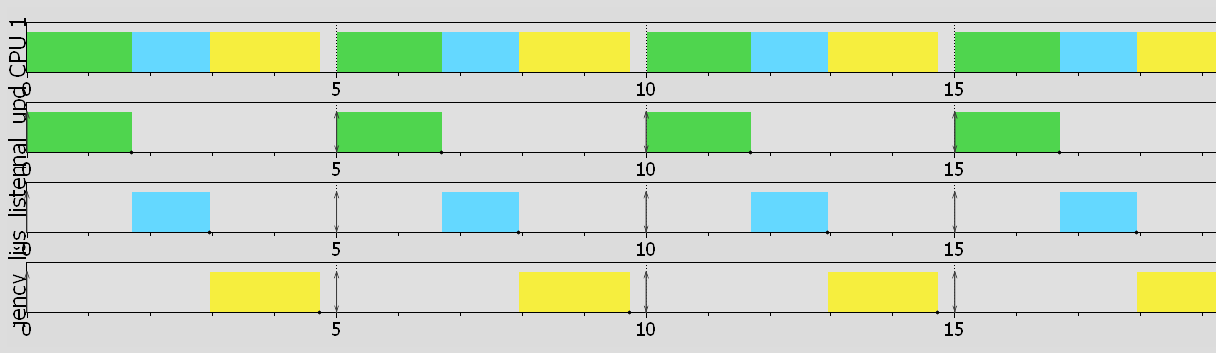
\includegraphics[width=0.5\textwidth]{images/schedule.png}
    \caption{Scheduler result.}
    \label{img:schedule}
\end{figure}

In the next section we will discussed how we verify and validate our system.




